% =====================================================================
\section{Part II: 25 Size and BE/ME Portfolios}
% =====================================================================

\paragraph{Sample.} 1969-07 to 2026-06, $T = 684$, $N = 25$. Estimates and
standard errors: percentage points per month. Mean market excess return:
$0.6116$.

\subsection{Question 1(b)}

\begin{table}[H]
\centering
\caption{Fama--MacBeth estimates ($t$-statistics test zero). Average monthly
cross-sectional R-squared: $0.2425$. Slope restriction
$E(\gamma_{M,t} - \mathrm{MktRF}_t) = 0$: mean difference $= -1.1873$,
SE $= 0.3916$, $t = -3.0316$, $p = 0.0025$.}
\small
\begin{tabular}{lrrrr}
\toprule
& Estimate & FMB SE & $t$-stat & $p$-value \\
\midrule
\texttt{gamma\_0} & 1.3554 & 0.3998 & 3.390 & 0.0007 \\
\texttt{gamma\_M} & $-0.5758$ & 0.4290 & $-1.342$ & 0.1800 \\
\bottomrule
\end{tabular}
\label{tab:p2b}
\end{table}

Using fixed full-period betas and 684 monthly cross-sectional regressions, we
obtain $\bar\gamma_0 = 1.3554$ (FMB SE $= 0.3998$, $t = 3.390$) and
$\bar\gamma_M = -0.5758$ (FMB SE $= 0.4290$, $t = -1.342$), in percent per
month. Standard errors use $\mathrm{sd}(\hat\gamma_{j,t})/\sqrt{T}$.

The significantly positive intercept rejects the zero-intercept restriction.
The slope also falls below the average market excess return of $0.6116\%$; the
difference has $t = -3.0316$ and $p = 0.0025$. These results reject the
Sharpe--Lintner CAPM restrictions and provide evidence against the proxy being
the tangency portfolio for these assets. The insignificant slope relative to
zero is not, by itself, grounds for rejection.

\subsection{Question 1(c)}

\begin{table}[H]
\centering
\caption{Fama--MacBeth and single cross-sectional regression estimates
compared. Cross-sectional R-squared: $0.1987$. $N = 25$.}
\small
\begin{tabular}{lrrrrrr}
\toprule
& FMB est. & FMB SE & FMB $t$-stat & OLS est. & OLS SE & OLS $t$-stat \\
\midrule
\texttt{gamma\_0} & 1.3554 & 0.3998 & 3.390 & 1.3554 & 0.2619 & 5.1759 \\
\texttt{gamma\_M} & $-0.5758$ & 0.4290 & $-1.342$ & $-0.5758$ & 0.2411 & $-2.3884$ \\
\bottomrule
\end{tabular}
\label{tab:p2c}
\end{table}

The single cross-sectional regression gives the same coefficients as
Fama--MacBeth: $\gamma_0 = 1.3554$ and $\gamma_M = -0.5758$, with
$R^2 = 0.1987$ and $N = 25$. Equality follows because the panel is balanced and
the regressors are fixed: averaging monthly OLS coefficients is equivalent to
regressing average returns on the same betas.

The OLS standard errors, $0.2619$ and $0.2411$, are smaller than the FMB
standard errors, $0.3998$ and $0.4290$. OLS measures dispersion around the
average-return regression, whereas FMB measures variation in monthly
coefficient estimates. FMB is preferable for inference on average premia here
because it incorporates that time-series variation and accommodates
contemporaneous correlation across portfolio returns. It does not eliminate
error from estimated betas.

\subsection{Question 1(d)}

\begin{figure}[H]
\centering
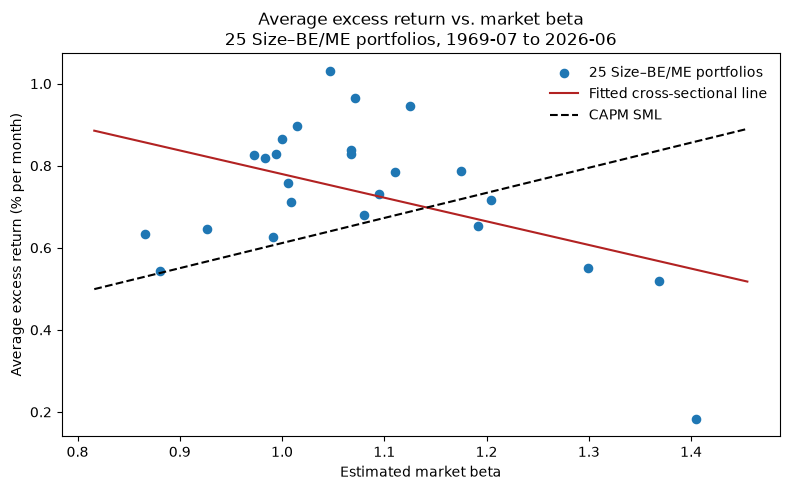
\includegraphics[width=0.78\textwidth]{Part2/figs/p2_1d_sml.png}
\caption{Average excess return against estimated market beta, 25
size--BE/ME portfolios. Fitted line: $1.3554 + (-0.5758) \times$ beta.
CAPM SML: $0.6116 \times$ beta. Cross-sectional R-squared: $0.1987$.}
\label{fig:p2d}
\end{figure}

The plot shows a negative fitted relationship:
\[
R^e_i = 1.3554 - 0.5758\,\hat\beta_{iM}.
\]
The CAPM instead predicts a line through the origin with positive slope
$0.6116$. The portfolios are widely scattered around the fitted line, with
$R^2 = 0.1987$, so market beta explains little of their average-return
variation. The plot is inconsistent with the predicted SML, although visual
evidence alone is not a formal statistical test.

\subsection{Question 1(f)}

\begin{table}[H]
\centering
\caption{Extended Fama--MacBeth estimates ($t$-statistics test zero). Average
monthly R-squared, beta only: $0.2425$; extended: $0.5288$. Slope restriction
$E(\gamma_{M,t} - \mathrm{MktRF}_t) = 0$: mean difference $= -0.8761$,
SE $= 0.2629$, $t = -3.3320$, $p = 0.0009$.}
\small
\begin{tabular}{lrrrr}
\toprule
& Estimate & FMB SE & $t$-stat & $p$-value \\
\midrule
\texttt{gamma\_0}    & 1.1539 & 0.3392 & 3.4017 & 0.0007 \\
\texttt{gamma\_M}    & $-0.2646$ & 0.3134 & $-0.8442$ & 0.3989 \\
\texttt{gamma\_size} & $-0.0194$ & 0.0302 & $-0.6428$ & 0.5206 \\
\texttt{gamma\_BM}   & 0.1573 & 0.0747 & 2.1055 & 0.0356 \\
\bottomrule
\end{tabular}
\label{tab:p2f}
\end{table}

With lagged characteristics included, the estimates are $\gamma_0 = 1.1539$
($t = 3.4017$), $\gamma_M = -0.2646$ ($t = -0.8442$),
$\gamma_{size} = -0.0194$ ($t = -0.6428$), and $\gamma_{B/M} = 0.1573$
($t = 2.1055$). Book-to-market has a positive premium significant at $5\%$,
while size is insignificant. Average monthly cross-sectional $R^2$ rises from
$0.2425$ to $0.5288$.

The positive book-to-market premium contradicts the CAPM prediction that
characteristics have no additional explanatory power after controlling for
beta. The intercept remains significantly positive, and the beta premium
remains below the market premium ($t = -3.3320$, $p = 0.0009$). Thus, adding
characteristics does not restore the Sharpe--Lintner CAPM restrictions.

Size is lagged one month and BE/ME uses the previous year's value, held
constant within each year. This follows the assignment's information-timing
convention and avoids using contemporaneous characteristics, though actual
accounting-data availability would require publication dates.

\subsection{Question 2}

\paragraph{2(a).} Using the 684 monthly observations from July 1969 to June
2026, we calculate the sample mean vector $\hat\mu$ and covariance matrix
$\hat\Sigma$ of the 25 portfolios' excess returns. The tangency weights are
\[
w_T = \frac{\hat\Sigma^{-1}\hat\mu}{\mathbf{1}'\hat\Sigma^{-1}\hat\mu}.
\]
The weights sum to one, with short selling allowed.

\begin{table}[H]
\centering
\caption{In-sample tangency weights and tangency betas. Weights are reported
as fractions of portfolio value. Size and BE/ME groups increase from 1 to 5.
Sum of weights: $1.000000$. Gross exposure (sum of absolute weights):
$13.3859$. Mean excess return: $2.5204\%$ per month. Monthly volatility:
$6.0461\%$. Monthly Sharpe ratio: $0.4169$. Weighted average beta:
$1.000000$.}
\small
\begin{tabular}{lrrlrr}
\toprule
Portfolio & Weight & Tang.\ beta & Portfolio & Weight & Tang.\ beta \\
\midrule
Size1\_BM1 & $-1.9858$ & 0.0725 & Size3\_BM4 & $-0.2411$ & 0.3253 \\
Size1\_BM2 & 0.6508 & 0.2841 & Size3\_BM5 & 0.2578 & 0.3834 \\
Size1\_BM3 & $-0.0034$ & 0.2903 & Size4\_BM1 & 1.1460 & 0.2595 \\
Size1\_BM4 & 0.9189 & 0.3563 & Size4\_BM2 & $-0.6837$ & 0.2694 \\
Size1\_BM5 & 0.9936 & 0.4092 & Size4\_BM3 & $-0.0040$ & 0.3006 \\
Size2\_BM1 & $-0.2076$ & 0.2061 & Size4\_BM4 & 0.4626 & 0.3274 \\
Size2\_BM2 & 0.8054 & 0.3119 & Size4\_BM5 & $-0.1819$ & 0.3330 \\
Size2\_BM3 & 0.2286 & 0.3289 & Size5\_BM1 & 0.7176 & 0.2484 \\
Size2\_BM4 & $-0.0409$ & 0.3435 & Size5\_BM2 & 0.0421 & 0.2559 \\
Size2\_BM5 & $-0.4743$ & 0.3749 & Size5\_BM3 & 0.5150 & 0.2519 \\
Size3\_BM1 & $-0.6186$ & 0.2183 & Size5\_BM4 & $-1.0900$ & 0.2154 \\
Size3\_BM2 & 0.0531 & 0.3109 & Size5\_BM5 & 0.4014 & 0.3288 \\
Size3\_BM3 & $-0.6615$ & 0.2819 &            &         &        \\
\bottomrule
\end{tabular}
\label{tab:p2w}
\end{table}

Gross exposure,
\[
\sum_i |w_i|,
\]
is $13.3859$, indicating substantial offsetting long and short positions.

\paragraph{2(b) Returns, betas, and cross-sectional results.} We construct the
tangency portfolio's monthly excess return using the same fixed weights
throughout:
\[
R^e_{T,t} = \sum_{i=1}^{25} w_{T,i} R^e_{i,t}.
\]
Its average excess return is $2.5204\%$ per month, monthly volatility is
$6.0461\%$, and the monthly Sharpe ratio is $0.4169$.

We estimate each portfolio's beta by regressing its excess returns on
$R^e_{T,t}$, including an intercept. Regressing average excess returns on these
new betas gives
\[
R^e_i \approx 0 + 2.5204\,\hat\beta_{i,T}, \qquad R^2 = 1, \qquad N = 25.
\]
The estimated intercept is effectively zero, while the slope equals the
tangency portfolio's average excess return. All 25 portfolios lie essentially
on the theoretical SML, so the fitted and theoretical lines overlap. The OLS
standard errors are effectively zero; the resulting $t$-statistics are not
economically meaningful because the fit is mechanically exact.

\begin{table}[H]
\centering
\caption{Cross-sectional regression using the in-sample tangency portfolio as
the market proxy. Cross-sectional R-squared: $1.000000$. $N = 25$. Mean
tangency excess return: $2.5204\%$ per month. Maximum absolute regression
residual: $9.659\times10^{-15}$. Fitted line: $0.0000 + (2.5204)\times$ beta.
CAPM SML: $2.5204\times$ beta.}
\small
\begin{tabular}{lrrr}
\toprule
& Estimate & OLS SE & $t$-stat \\
\midrule
\texttt{gamma\_0} & $4.83988\times10^{-15}$ & $4.34718\times10^{-15}$ & 1.11334 \\
\texttt{gamma\_M} & 2.52036 & $1.45191\times10^{-14}$ & $1.7359\times10^{14}$ \\
\bottomrule
\end{tabular}
\label{tab:p2q2}
\end{table}

\begin{figure}[H]
\centering
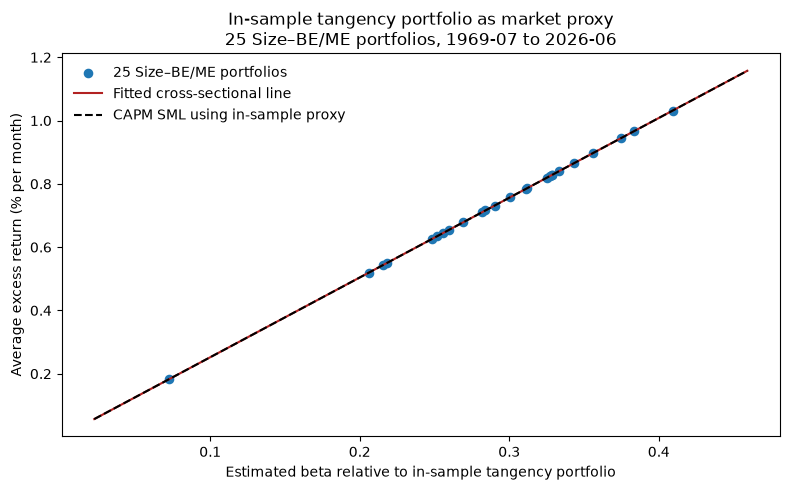
\includegraphics[width=0.78\textwidth]{Part2/figs/p2_q2_insample.png}
\caption{Average excess return against beta estimated against the in-sample
tangency portfolio. Fitted line: $0.0000 + (2.5204)\times$ beta. CAPM SML:
$2.5204\times$ beta.}
\label{fig:p2q2}
\end{figure}

\paragraph{2(c).} This perfect fit does not independently support the CAPM. The
tangency portfolio is constructed to be mean--variance efficient using the same
assets and observations used in the regression. Its weights satisfy
\[
w_T \propto \hat\Sigma^{-1}\hat\mu,
\]
which implies
\[
\hat\mu_i = \hat\beta_{i,T}\,\hat\mu_T .
\]
Thus, the zero intercept, matching slope, and perfect fit follow from portfolio
mathematics.

This illustrates Roll's critique: CAPM tests depend on whether the chosen
market proxy is mean--variance efficient. The true market portfolio includes
all wealth and is not directly observable. Rejecting the CAPM with a particular
proxy could therefore reflect a poor proxy, while obtaining a perfect fit with
a deliberately constructed tangency portfolio does not establish that the true
market portfolio is efficient.

\subsection{Question 3}

\paragraph{3(a).} Sample 1 contains odd-numbered months in even years and
even-numbered months in odd years, giving 342 observations. Using only these
observations, we estimate the mean vector and covariance matrix of excess
returns and calculate
\[
w_1 = \frac{\hat\Sigma_1^{-1}\hat\mu_1}{\mathbf{1}'\hat\Sigma_1^{-1}\hat\mu_1}.
\]
The weights sum to 1, with gross exposure $\sum_i |w_{1,i}| = 15.4800$ and
individual weights ranging from $-1.6671$ to $1.4736$. We hold these weights
fixed and apply them to the 342 months in Sample 2. These returns are out of
sample because none of the evaluation observations were used to estimate the
weights.

\paragraph{3(b).} Sample 2 contains even-numbered months in even years and
odd-numbered months in odd years, also giving 342 observations. We estimate a
separate tangency portfolio using only Sample 2's mean vector and covariance
matrix, with the same normalization.

These weights sum to 1, have gross exposure of $17.2082$, and range from
$-2.4853$ to $1.3680$. We then apply them, unchanged, to Sample 1 returns. This
reverses the estimation and evaluation samples, ensuring that neither half is
evaluated using weights estimated from itself. The checks confirm that the
samples do not overlap and together cover all 684 months.

\begin{table}[H]
\centering
\caption{Out-of-sample tangency weights. Sample 1: 342 months; Sample 2: 342
months; total 684 months, no overlap and complete coverage.}
\small
\begin{tabular}{llrrrr}
\toprule
Estimated from & Applied to & Weight sum & Gross exposure & Min weight & Max weight \\
\midrule
Sample 1 & Sample 2 & 1.0 & 15.4800 & $-1.6671$ & 1.4736 \\
Sample 2 & Sample 1 & 1.0 & 17.2082 & $-2.4853$ & 1.3680 \\
\bottomrule
\end{tabular}
\label{tab:p2oosw}
\end{table}

\paragraph{3(c).} We combine Sample 1 returns generated with $w_2$ and Sample 2
returns generated with $w_1$, then sort them chronologically. The resulting OOS
tangency series covers July 1969--June 2026 and has a mean excess return of
$1.9754\%$ per month, monthly volatility of $7.0300\%$, and monthly Sharpe
ratio of $0.2810$.

We use this combined excess-return series as the market proxy and estimate each
portfolio's beta through a full-period time-series regression with an
intercept. The cross-sectional regression of average excess returns on these
betas is
\[
R^e_i = 0.0684 + 3.2851\,\hat\beta_{i,\mathrm{OOS}} + \hat\eta_i .
\]

\begin{table}[H]
\centering
\caption{Cross-sectional regression using the out-of-sample tangency portfolio
as the market proxy. Returns are measured in percent per month. The regression
has $R^2 = 0.9753$ and $N = 25$. Mean OOS market excess return: $1.9754\%$ per
month.}
\small
\begin{tabular}{lrrr}
\toprule
Coefficient & Estimate & OLS standard error & $t$-statistic \\
\midrule
$\gamma_0$ & 0.0684 & 0.0228 & 2.9930 \\
$\gamma_M$ & 3.2851 & 0.1091 & 30.1058 \\
\bottomrule
\end{tabular}
\label{tab:p2q3}
\end{table}

\begin{figure}[H]
\centering
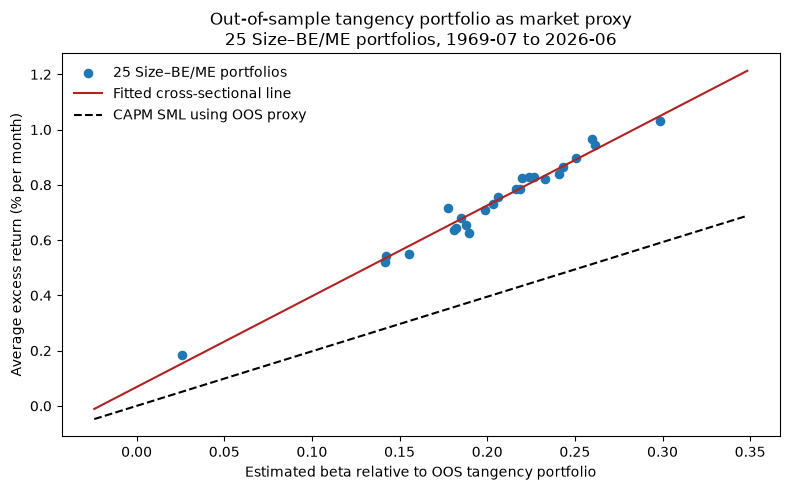
\includegraphics[width=0.78\textwidth]{Part2/figs/p2_q3_oos.png}
\caption{Average excess return against beta estimated against the
out-of-sample tangency portfolio. Fitted line: $0.0684 + (3.2851)\times$ beta.
CAPM SML: $1.9754\times$ beta.}
\label{fig:p2q3}
\end{figure}

The plot shows a strong positive relationship: the portfolios cluster closely
around the fitted line, which explains $97.53\%$ of the cross-sectional
variation in average excess returns. However, the fitted line lies above the
theoretical SML, whose intercept is zero and slope is $1.9754$. Thus, a close
fit to the estimated line does not establish that the CAPM restrictions hold.
The reported slope $t$-statistic tests equality to zero, not equality to
$1.9754$.

Each month's return is excluded from the sample used to estimate its portfolio
weights. Because the two samples are interleaved in time, this is a
held-out-sample exercise rather than a strictly forward-looking trading
backtest.

\subsection{Question 4}

\paragraph{1. Comparing the results.}

\begin{table}[H]
\centering
\caption{In-sample and out-of-sample tangency proxies compared.}
\small
\begin{tabular}{lrr}
\toprule
Statistic & Q2: In-sample & Q3: Out-of-sample \\
\midrule
$\gamma_0$ (SE, $t$) & $4.84\times10^{-15}$ & 0.0684 \\
 & ($4.35\times10^{-15}$, $t = 1.11$) & (0.0228, $t = 2.99$) \\
$\gamma_M$ (SE, $t$) & 2.5204 & 3.2851 \\
 & ($1.45\times10^{-14}$, $t = 1.74\times10^{14}$) & (0.1091, $t = 30.11$) \\
Proxy mean excess return (CAPM slope) & 2.5204 & 1.9754 \\
$\gamma_M \div$ proxy premium & 1.00 & 1.66 \\
Cross-sectional $R^2$ & 1.000000 & 0.9753 \\
Max absolute residual & $9.66\times10^{-15}$ & not reported \\
Proxy Sharpe ratio (monthly) & 0.4169 & 0.2810 \\
\bottomrule
\end{tabular}
\label{tab:p2q4}
\end{table}

\begin{tight}
\item $\gamma_0$: In Q2 the intercept is zero to machine precision. The
$t = 1.11$ is rounding noise, not a meaningful test. In Q3 the intercept is
$0.0684\%$ per month, about $0.82\%$ per year, with $t = 2.99$, indicating a
statistically significant common pricing error across the 25 portfolios.

\item $\gamma_M$: In Q2 the slope equals the proxy's premium exactly,
$2.5204$. In Q3 the slope is $3.2851$, about $1.66$ times the proxy premium of
$1.9754$. The raw slopes should not be compared directly across Q2 and Q3
because each set of betas is measured against a different proxy. What matters
for the CAPM is whether the slope equals that proxy's own premium. It does in
Q2 but not in Q3.

\item Standard errors: Q2's standard errors are essentially zero because the
regression residuals are essentially zero, so the enormous slope $t$-statistic
is not economically informative. Q3's $t$-statistics use ordinary
cross-sectional OLS standard errors, which do not account for beta-estimation
error or cross-portfolio dependence. Also, $t = 30.11$ tests $\gamma_M = 0$,
not the CAPM restriction $\gamma_M = 1.9754$.

\item SML shape: In Q2 the fitted line,
$R^e_i = 0.0000 + 2.5204\beta_i$,
and the theoretical SML are the same line. In Q3 the fitted line,
$R^e_i = 0.0684 + 3.2851\beta_i$,
has both a higher intercept and a steeper slope than the theoretical SML,
$R^e_i = 1.9754\beta_i$. Thus, for positive betas, the fitted Q3 line lies
above the theoretical SML.

\item Which is cleaner? Q2 fits the CAPM restrictions mechanically: the
intercept is zero, the slope equals the proxy premium, and $R^2 = 1$. Both Q2
and Q3 fit much better than the value-weighted market proxy in Part I, where
$\gamma_0 = 1.3554$, $\gamma_M = -0.5758$, and $R^2 = 0.1987$.
\end{tight}

\paragraph{2. Why Q2 and Q3 differ, and the link to Roll (1977).}

\textbf{The in-sample proxy is efficient by construction.} Using excess
returns, the tangency weights are
\[
w_T = \frac{\hat\Sigma^{-1}\hat\mu}{\mathbf{1}'\hat\Sigma^{-1}\hat\mu}.
\]
Let
\[
c = \mathbf{1}'\hat\Sigma^{-1}\hat\mu.
\]
Then the result follows in four steps:
\begin{enumerate}\setlength{\itemsep}{2pt}\setlength{\topsep}{3pt}
\item Rearranging the tangency-weight formula gives
$\hat\Sigma w_T = \hat\mu / c$.
\item $\hat\Sigma w_T$ is the vector of sample covariances between each
portfolio and the tangency portfolio:
$\widehat{\mathrm{Cov}}(R_i, R_T)$.
\item The tangency portfolio's variance is
$w_T'\hat\Sigma w_T = \hat\mu_T / c$.
\item Therefore,
\[
\hat\beta_i = \frac{\widehat{\mathrm{Cov}}(R_i, R_T)}
{\widehat{\mathrm{Var}}(R_T)} = \frac{\hat\mu_i}{\hat\mu_T},
\qquad\text{which implies}\qquad
\hat\mu_i = \hat\beta_i \hat\mu_T .
\]
\end{enumerate}
This identity holds for every portfolio.

Q2 estimates the weights using the same 684 months and the same 25 portfolios
that are subsequently used in the CAPM test. Because the OLS betas are also
based on the same sample covariances and variances, the beta-pricing identity
must hold essentially exactly. The maximum residual of $9.66\times10^{-15}$
confirms this.

\textbf{Why the CAPM can look successful even when the market is mismeasured.}
Roll's critique is that an empirical CAPM test is fundamentally a test of
whether the chosen market proxy is mean-variance efficient. The true CAPM
market portfolio contains all relevant wealth and cannot be directly observed.

The results illustrate the problem. With the observable value-weighted market
proxy in Part I, the CAPM performs poorly. With a proxy constructed directly
from the test assets in Q2, the fit becomes perfect. Nothing about the true
market changed; only the proxy changed.

Therefore, Q2's apparent success mainly shows that the proxy was constructed to
be mean-variance efficient relative to these 25 portfolios in this sample. A
perfect fit does not independently establish that the true market portfolio is
efficient, while rejection using another proxy could reflect proxy error rather
than failure of the CAPM itself.

\textbf{Why the out-of-sample version is more informative.} In Q3, each month's
proxy return uses tangency weights estimated from the opposite half of the
data. Therefore, the means and covariances used to construct the proxy are no
longer the same moments used to evaluate it. The exact in-sample identity above
no longer has to hold.

Estimation error therefore becomes important:
\begin{tight}
\item Inverting the $25\times25$ covariance matrix in
$\hat\Sigma^{-1}\hat\mu$
can magnify estimation noise.
\item This produces large long and short positions. Gross exposure is $15.48$
and $17.21$ in the two estimation samples, with individual weights ranging
roughly from $-2.4853$ to $1.4736$.
\item Weights optimized using one half of the data may partly fit noise
specific to that half. When applied to the other half, performance
deteriorates. The proxy mean falls from $2.5204\%$ to $1.9754\%$ per month,
volatility rises from $6.0461\%$ to $7.0300\%$, and the monthly Sharpe ratio
falls from $0.4169$ to $0.2810$.
\item Because the OOS proxy is no longer guaranteed to lie on the
evaluation-sample mean-variance frontier, pricing errors appear:
$\gamma_0 > 0$, the fitted slope differs from the proxy premium, and
$R^2 < 1$.
\end{tight}

The remaining high $R^2$ of $0.9753$ indicates that the beta-return relation
remains strong out of sample, even though the exact in-sample CAPM identity
disappears.

Limits of the Q3 test:
\begin{tight}
\item The two samples alternate months and therefore span the same broad
economic periods, so this is a relatively mild out-of-sample test.
\item The second-pass average returns and betas are calculated using the
combined sample, so the design is not equivalent to a completely separate
future holdout period.
\item The OOS proxy is still constructed from the same 25 test portfolios
rather than from the true aggregate market portfolio. Therefore, Q3 makes the
test more informative but does not eliminate Roll's critique.
\end{tight}

\paragraph{3. Evaluating the LLM explanation.}

\textbf{1. Did it predict a steeper SML and lower pricing errors?} Partly.

The LLM correctly predicted that an in-sample tangency proxy would generate
small pricing errors and a very strong beta-return relationship. It actually
understated the strength of the result: it called the exercise ``almost
tautological,'' while Q2 produces an essentially exact fit with
$R^2 = 1.000000$.

However, it did not explicitly predict a steeper SML. In fact, ``steeper'' is
not the key criterion. Q3's fitted slope, $3.2851$, is numerically steeper than
Q2's $2.5204$. The important CAPM restriction is instead whether the fitted
slope equals the proxy's own mean excess return. That equality holds exactly in
Q2 but fails in Q3.

\textbf{2. Did it explain why the portfolio is efficient by construction?} Yes.
This is the strongest part of the LLM explanation.

It correctly argues that the tangency first-order condition implies
\[
\mu - r_f\mathbf{1} \propto \Sigma w_T ,
\]
and recognizes that $\Sigma w_T$ is the vector of covariances between each test
asset and the tangency portfolio. This leads directly to beta pricing.

There are two minor precision issues:
\begin{tight}
\item It skips the intermediate step needed to determine the proportionality
constant. Premultiplying by $w_T'$ gives the connection between the constant,
the tangency portfolio premium, and its variance.
\item It writes the result using population expectations such as $E[R_i]$,
whereas the exact identity here is an \emph{in-sample} identity involving
sample moments, such as $\hat\mu_i$. This distinction explains why the Q2 fit
is exact in the observed sample but need not hold out of sample.
\end{tight}

\textbf{3. Did it anticipate why the out-of-sample results could deteriorate?}
In general terms, yes. The LLM correctly explained that moments in the
evaluation sample need not equal the moments used to estimate the weights, so
mean-variance efficiency is no longer guaranteed.

However, its explanation was less complete about the empirical pattern observed
in Q3. It did not emphasize:
\begin{tight}
\item estimation error amplified by $\hat\Sigma^{-1}$;
\item the resulting extreme leveraged weights;
\item the lower out-of-sample Sharpe ratio;
\item the positive intercept and slope exceeding the proxy premium;
\item the fact that $R^2$ nevertheless remains high at $0.9753$;
\item the exact two-way sample-splitting procedure used in Q3;
\item or the fact that the OOS proxy is still not the true market portfolio, so
Roll's critique remains relevant.
\end{tight}

Overall, the LLM's explanation is conceptually correct and explains the exact
in-sample fit in Q2 well. It is less complete in explaining the magnitude and
specific pattern of the deterioration observed in Q3.
